\section{Arhitektura sistema}
U ovom poglavlju biće prikazan predlog arhitekture sistema za socijalnu mrežu. 
\begin{itemize}
    \item Izabrana je Veb aplikacija zbog veće dostupnosti, za svakog korisnika je dovoljno da ima internet mrežu i računar ili mobilni telefon. 
    \item Interfejs socijalne mreže pruža korisnicima lako i jednostavno korišćenje.
    \item Pored dostupnosti, lakog i jednostavnog korišćenja bitna je i ažurnost, prilikom neke promene svi korisnici će ubrzo nakon toga videti samu promenu. 
    \item Arhitektura obezbeđuje administratoru da ukoliko izgubi internet konekciju može nastaviti sa radom preko lokalne mreže.
\end{itemize}

\subsection{Karakteristike arhitekture}
	\begin{enumerate}
		\item Tip aplikacije - Veb aplikacija
		\item Strategija isporučivanja - Više klijentskih i jedan serverski računar
		\item Tehnologije - HTML5, CSS, JavaScript, PHP
		\item Prateće komponente - Bekap baze podataka 
	\end{enumerate}

\subsection{Slojevi arhitekture}
\begin{enumerate}
    \item Prezentacioni sloj - najniži sloj, koji korisniku omogućava sto udobnije korišćenje Veb-aplikacije
    \item Komunikacioni sloj - deli se na dva podsloja:
    \begin{enumerate}
	    \item Klijent kontroler - komunicira sa serverskim slojem arhitekture i obaveštava prezentacioni sloj o njegovoj akciji
	    \item Server kontroler - ima sličnu ulogu kao klijentski sloj arhitekture, ali pored toga ima mogucnost komunikacije sa bazom podataka
	\end{enumerate}
    \item Sloj podataka - omogućava serverskom sloju da pristupa bazi podataka
\end{enumerate}
\begin{figure}[h!]
		\centerline{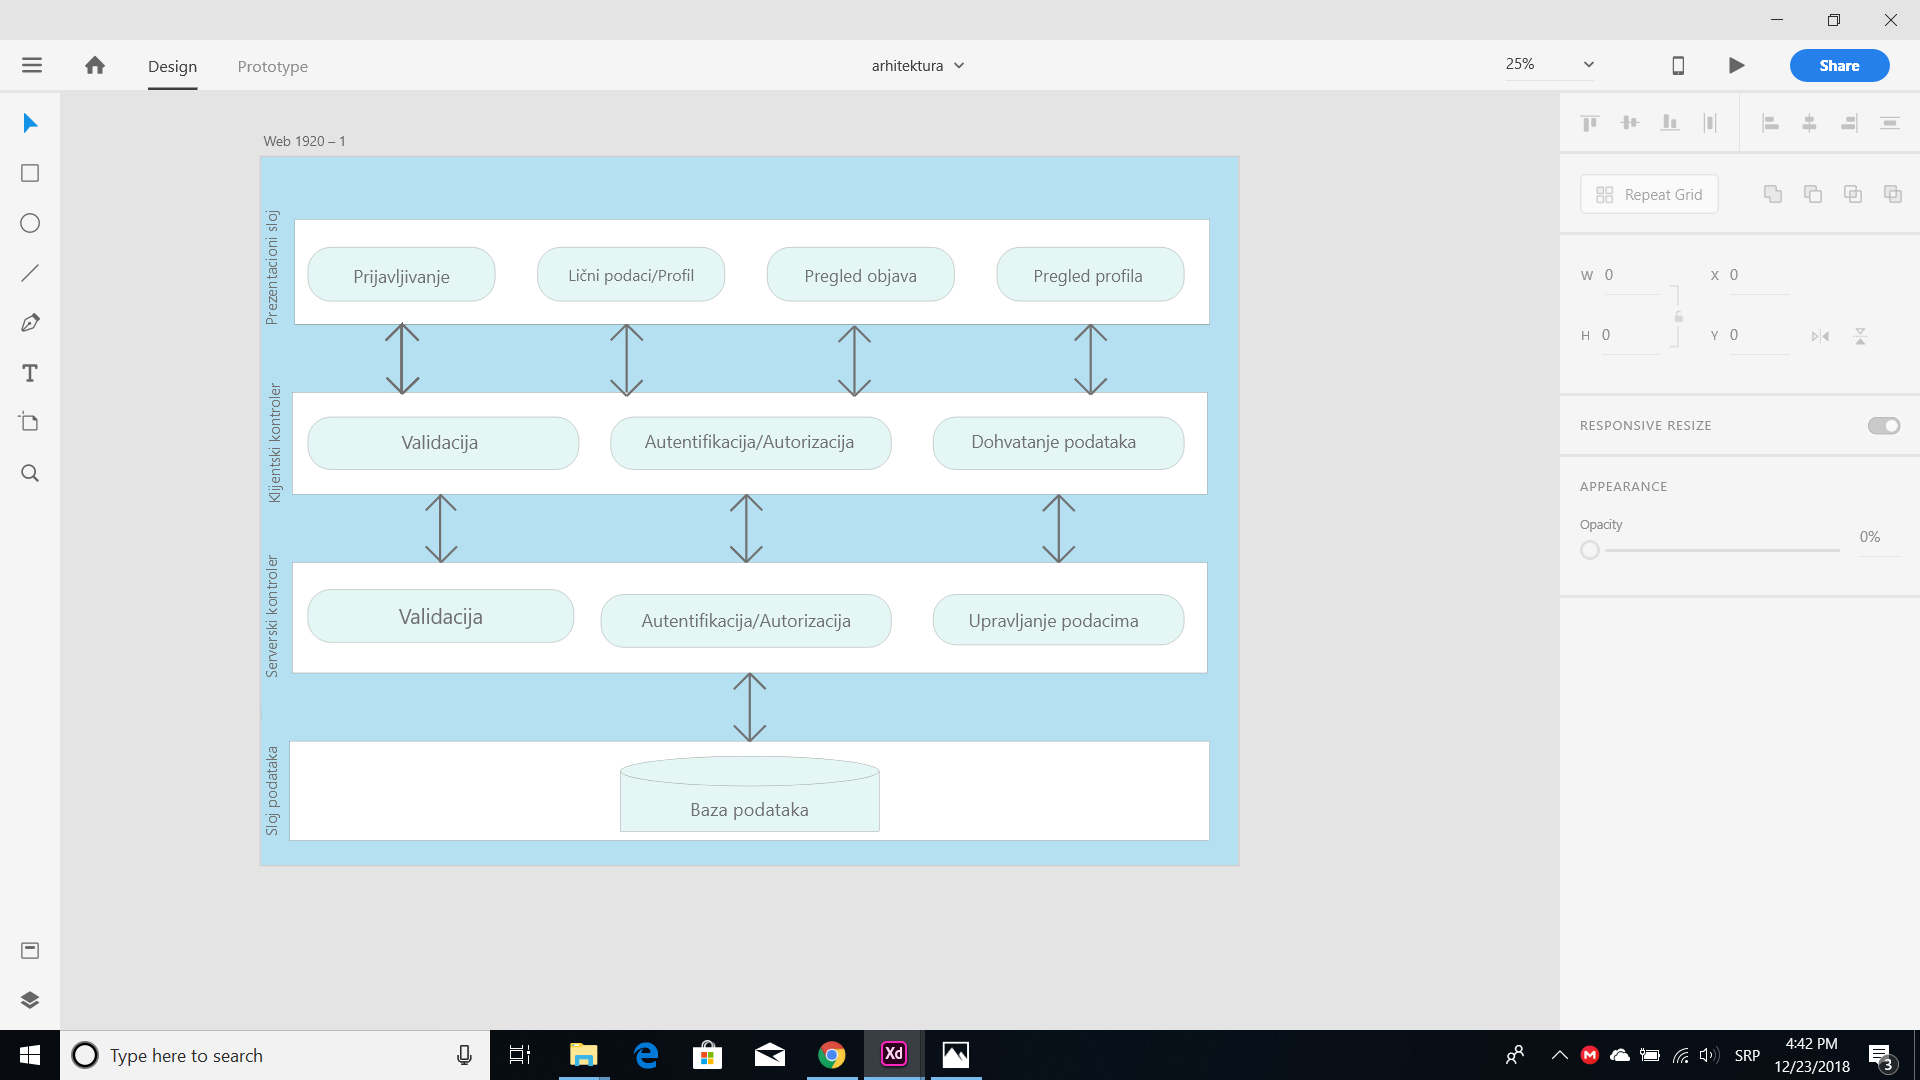
\includegraphics[scale=0.7]{slike/arhitektura.png}}
		\captionof{figure}{Predlog arhitekture}
\end{figure}
